\vspace{-30pt}
\begin{figure}[h]
    \centering
    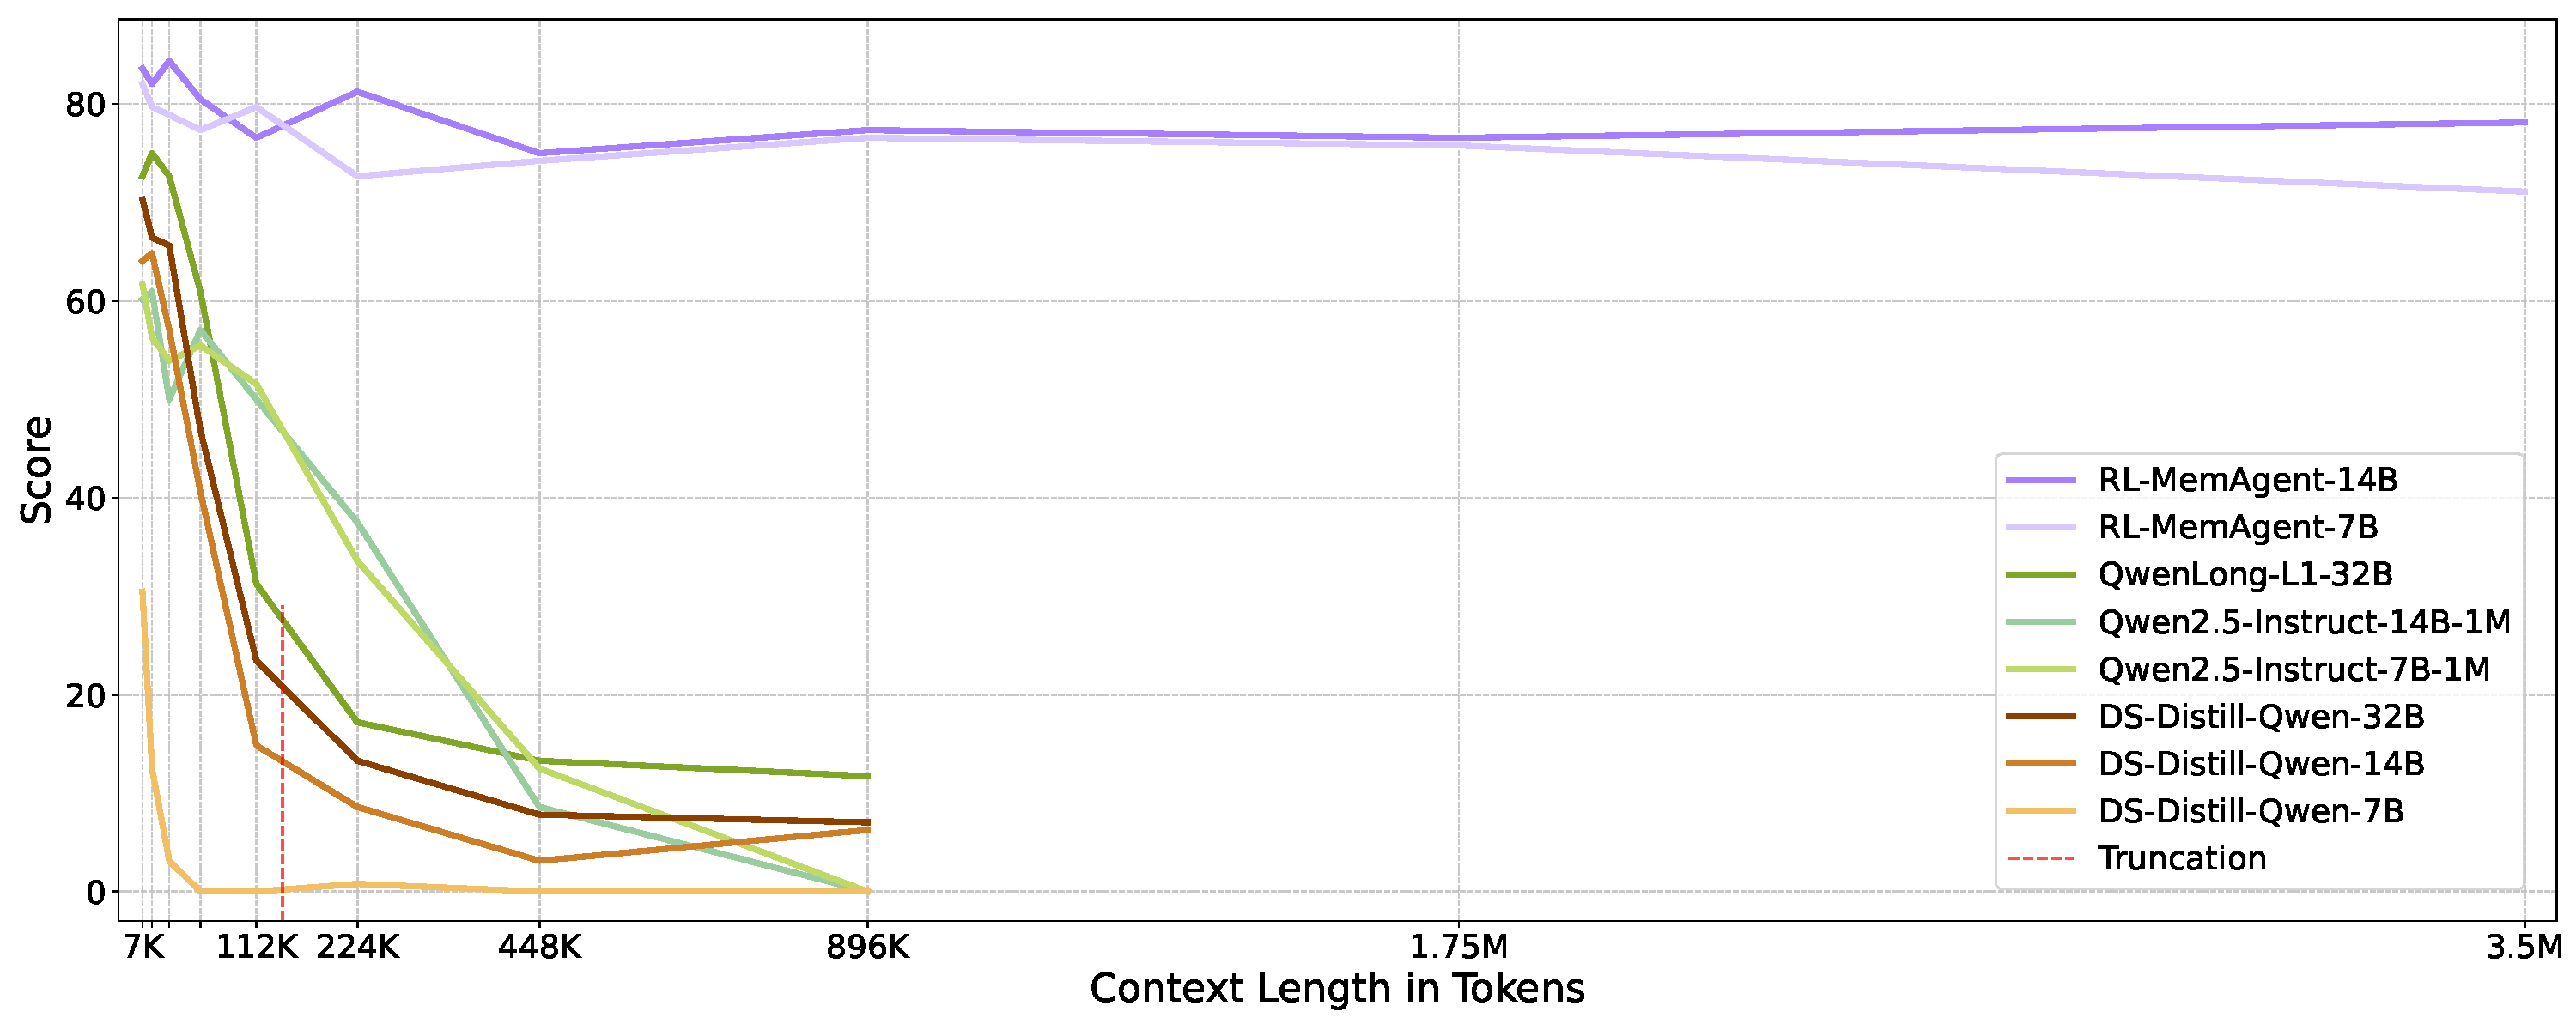
\includegraphics[width=0.95\linewidth]{figs/main_result.pdf}
    \caption{Accuracy scores of RULER-HotpotQA~~\cite{hsieh2024ruler, yang2018hotpotqa} . Even models that employ long-context continual pretraining and extrapolation techniques fail to maintain consistent performance. In contrast, \method with RL demonstrates nearly lossless performance extrapolation.}
    \label{fig:front}
\end{figure}

\newpage

\section{Introduction}

While having demonstrated impressive capabilities~\cite{o1,gemini-thinking,grok,claude35sonnet,gpt4}, industry-level Large Language Model (LLM) systems~\cite{claude4,li2025minimax,liu2024deepseek} still face a critical challenge: how to handle long contexts effectively - processing an entire book, executing a complex chain of reasoning over many steps, or managing the long-term memory of an agent system - all these complex tasks can generate overflowing text that quickly explodes the typical-size context window of current LLMs.

Existing approaches to long-context tasks are three-pronged. The first involves length extrapolation methods by shifting the positional embeddings in order to extend the context window of the model~\cite{su2024roformer, blocntkaware,chen2023extending, peng2023yarn, an2024training}, plus continued pre-training~\cite{liu2023scaling, xiong2023effective, gao2025nextlong}. Despite promising potential, these methods often suffer from performance degradation and slow processing speed due to $O(n^2)$ computational complexity when applied to extremely long text. The second school of methods leverages sparse attention~\cite{beltagy2020longformer, zhao2019explicit, xiao2023efficient} and linear attention mechanisms~\cite{child2019generating, katharopoulos2020transformers} to reduce the complexity of attention for more efficient processing of longer sequences. However, this typically requires training from scratch, with inherent adversities such as linear attention facing difficulties in parallel training or sparse attention depending on human-defined patterns. The last line of inquiry investigates context compression~\cite{jiang2023llmlingua, li2023compressing, behrouz2024titans, zhang2024test}, which aims to condense information in token-level or external-memory-plugin modules. Such approaches often struggle with extrapolation, and require the integration of additional modules or context operations, which ineluctably disrupts the standard generation process and hinders compatibility as well as parallelization. 

Hence, a successful LLM with strong long-context capabilities requires the trinity of:
$1)$ processing infinite length of text; 
$2)$ scaling without performance drop; and $3)$ efficient decoding with linear complexity. To pursue this quest, we return to the basic intuition behind long-context modeling~\cite{miller1956magical, hochreiter1997long, graves2014neural, weston2014memory}. When humans process long-context information, we tend to abstract out the main revealing conceptions to capture the essence of the whole text, often by making notes of critical details or using short-handed stenograph to record the key points, while discarding redundant and irrelevant data. We do not attempt to memorize every single fact or each small piece of information; instead, we focus our intellectual energy on more important aspects of the task at hand. This selective attention not only simplifies the process but also aids in tackling complex problems more efficiently. 
 

Following this anthropocentric intuition, we propose a novel use of Reinforcement Learning (RL) to equip LLMs with a dynamically updated fixed-length `memory', as illustrated in \autoref{fig:workflow}. During inference, the LLM processes the input text segment-by-segment. As it reads each segment, the model proactively and selectively updates the memory, which then contributes to the generation of the final output after all relevant messages are aggregated and synergized in the memory. This clever mechanism allows the LLM to flexibly handle arbitrary text lengths while maintaining a linear time complexity during processing, since the length of the memory is fixed, which leads to a fixed context window size for the model. This segment-based approach generates multiple outputs from a single long-text input, requiring multiple rounds of memory updates and a final round for the generation of the final response. Training this type of agent workflow, which enables dialogues across multiple independent contexts, is still an unexplored territory in current LLM study. Existing systems typically handle workflow trajectories via alternating tool calls or environment feedback by either simply concatenating \cite{Agent-R1,jin2025search} them  or using a sliding window \cite{feng2025group} approach, which lacks flexibility and scalability in practice. 
Our \method approach, instead, proposes that treats each context-independent conversation as an optimization objective. Based on the DAPO\cite{yu2025dapo} algorithm, we implement the Multi-Conv DAPO to optimize an arbitrary agent workflow by verifiable outcome reward.

In our experiments, an RL-trained model with a modest 8K context window (with a 1024-token memory and a 5000-token document chunk) trained on 32K documents exhibits consistently superb capabilities for Question Answering (QA) tasks on documents of up to 4 million tokens,  without performance drop and with linear computation cost. This demonstratively showcases the efficiency and scalability of our long-context memory approach.

Our major contributions are threefold:

\begin{itemize}
\item We introduce a novel approach that enables LLMs to process arbitrarily long inputs within limited context window under linear time complexity during inference, overcoming a significant bottleneck in long-context processing. 

\item We design an agent workflow to implement this mechanism and propose an end-to-end training approach using the multi-conversation DAPO algorithm.

\item We empirically demonstrate that our RL-trained  method allows models to extrapolate to vastly long documents with minimal performance degradation, pushing the boundaries of what is currently achievable in long-context LLM systems.
\end{itemize}


\begin{figure}[t]
    \centering
    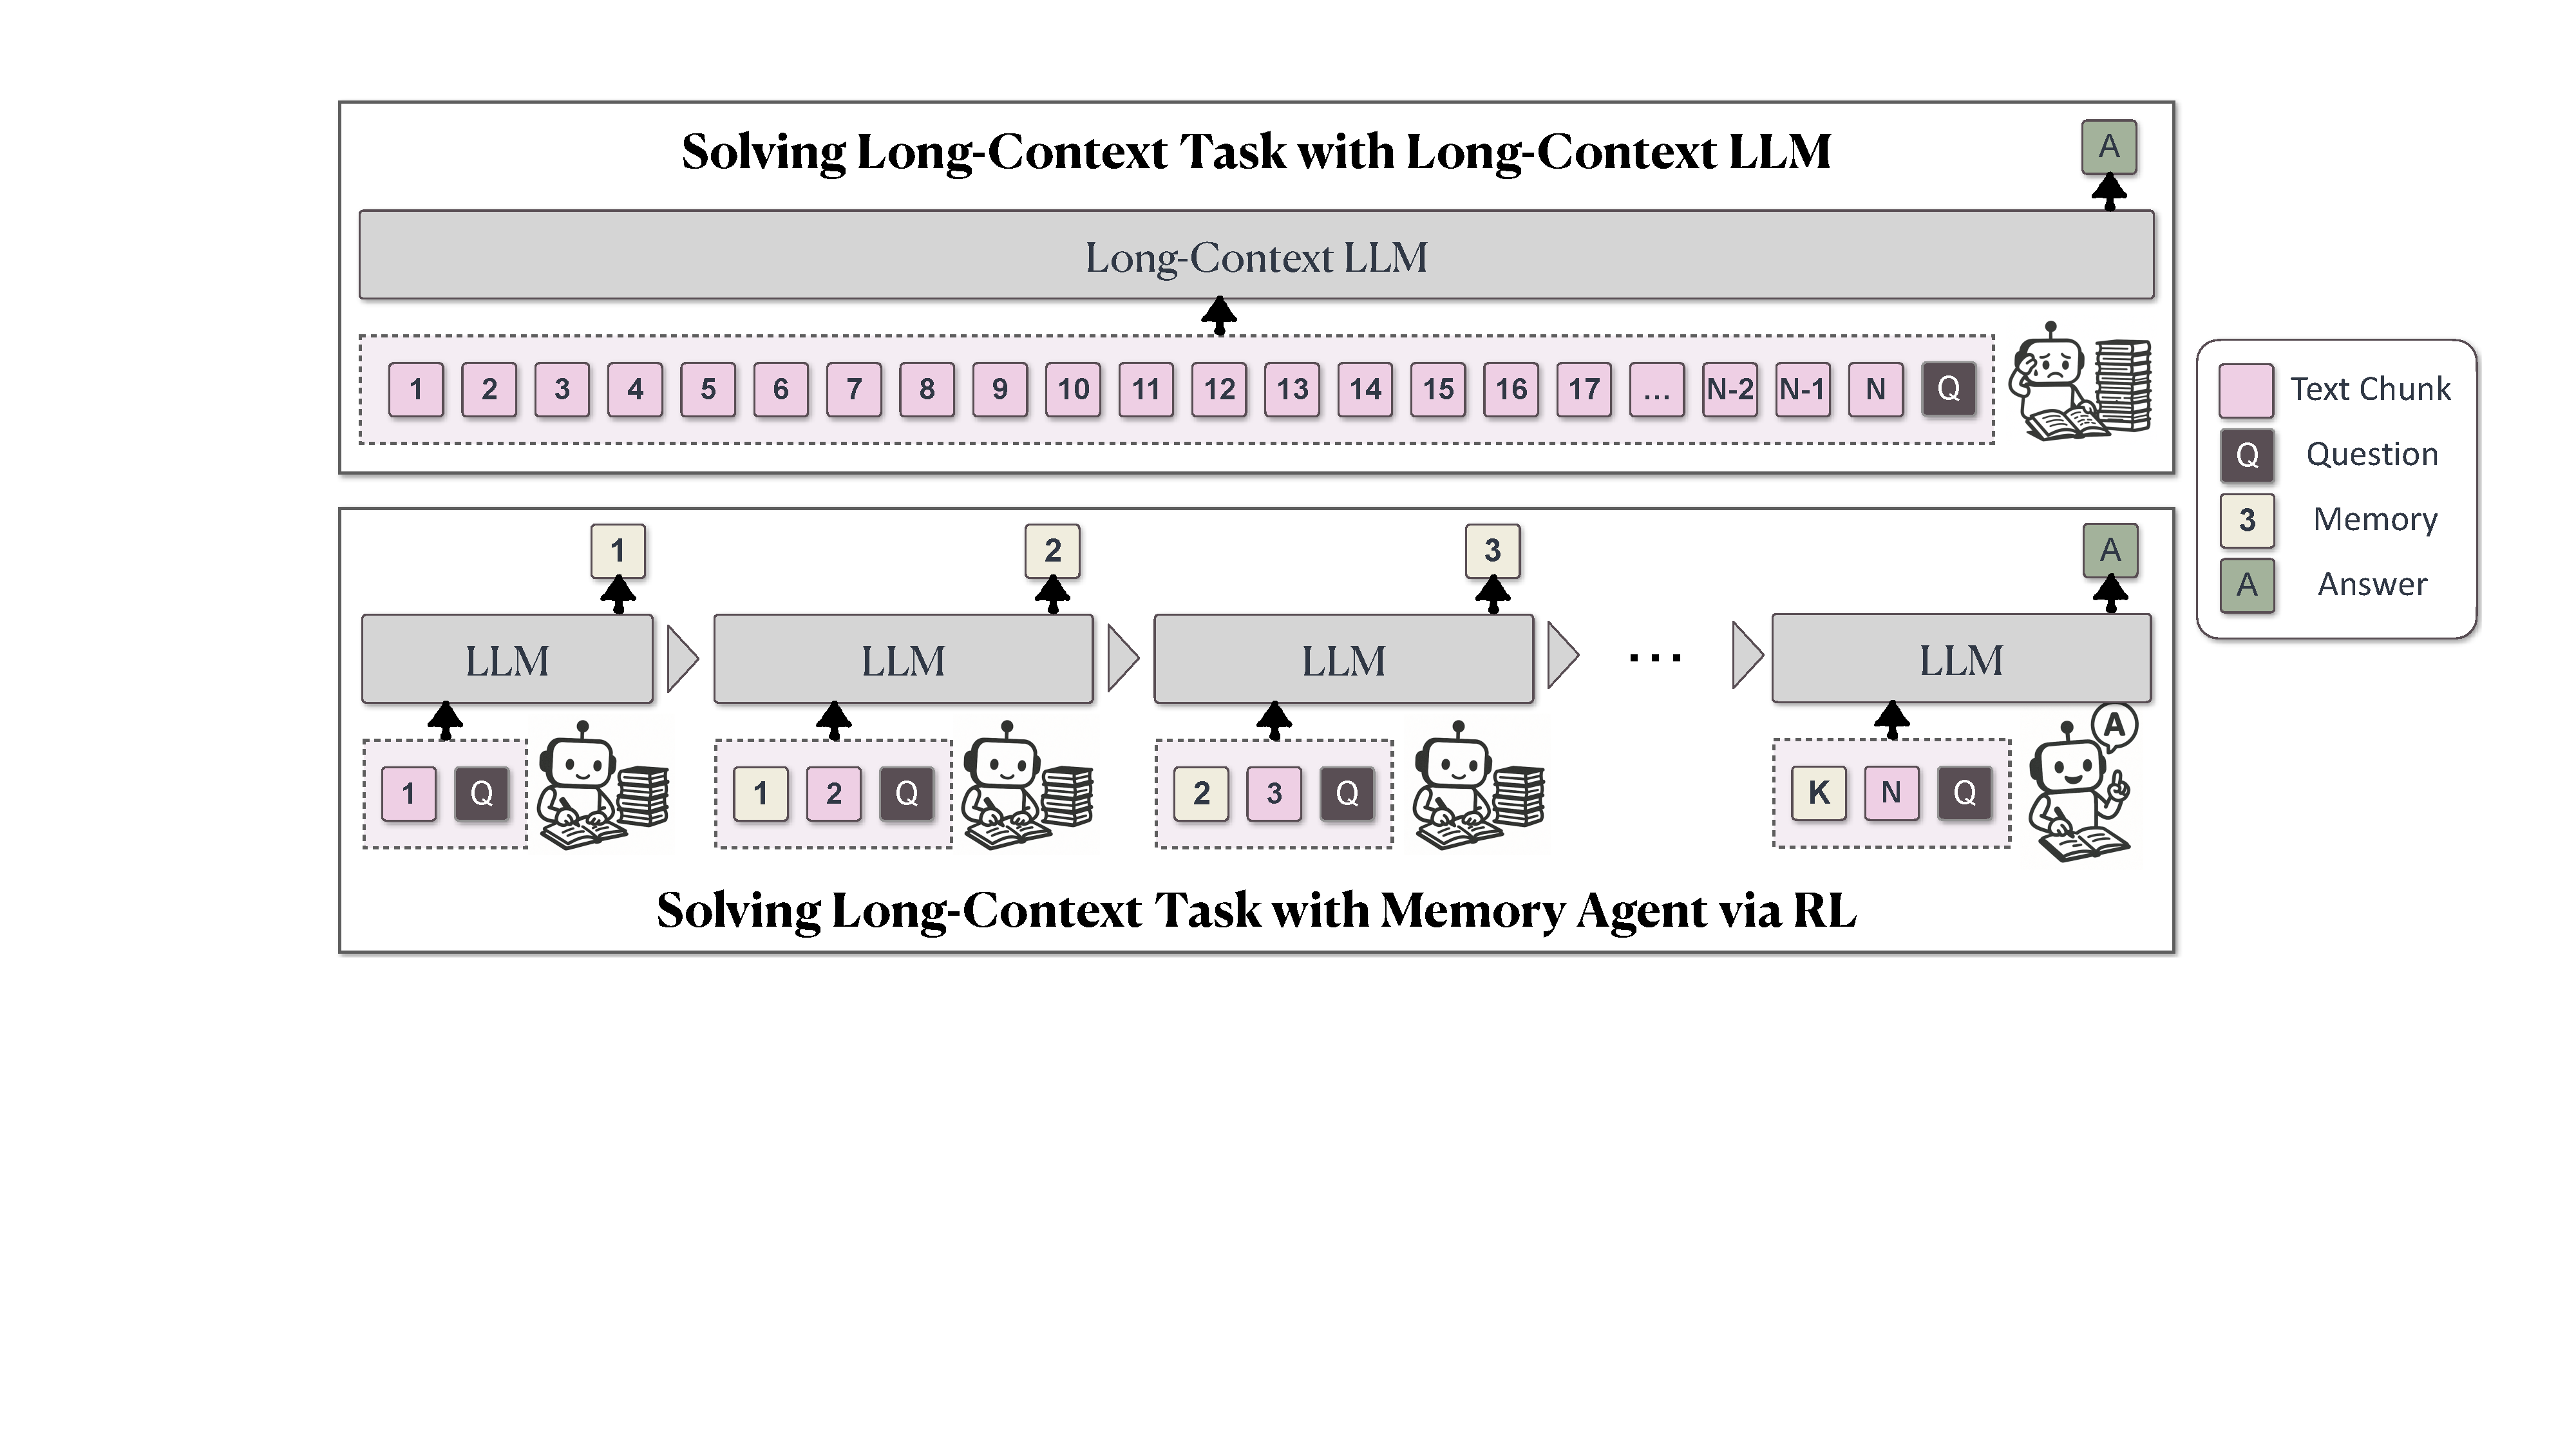
\includegraphics[width=0.95\linewidth]{figs/method.pdf}
    \caption{\method is inspired by the way humans process long documents. It divides the document into multiple chunks and allows LLMs to process them iteratively, recording relevant information in memory. Finally, LLMs generate answers based on the information stored in the memory.}
    \label{fig:workflow}
\end{figure}
